\chapter{Problem description}

In this chapter we will discuss the necessity of a tool like Gocey, followed by a brief overview of the concepts involved on this project.

\section{The necessity of a distributed system for collaborative science}
Nowadays, computers play an essential role in scientific research. For most scientists, a desktop machine is enough to store and process the data they work with, but a considerable amount of them need supercomputers to be able to deal with more complex problems \cite{computing-in-science}.

Supercomputers are expensive, and price ranges vary widely depending on the computational capacities of the system; For example, a supercomputer with a power of 40 TFLOPS like \textit{Alhambra}, the supercomputer at the \textit{University of Granada}, costs around \$670,000\cite{ideal-alhambra}. A supercomputer leading the list Top500,  like the one from \textit{Oak Ridge National Laboratory}, with 200 PetaFLOPS manufactured by IBM costs \$200 million\cite{oak-ridge}. Hence having access to one of these machines is not common.

Distributed systems are an attractive alternative to supercomputers. A distributed system can be defined as a set of independent machines that interact with each other, cooperating to achieve a common objective. Even though this approach is much cheaper than using a supercomputer, an important investment is required in order to buy and set up these machines.

In 2002, the \textit{University of California, Berkeley} addressed the problem described above by developing \textit{BOINC}\cite{boinc-website}, a platform for volunteer computing where users can contribute to different scientific projects with their computers or smart-phones. As of June 2019 the platform has achieved a power of over 27 PetaFLOPS in the last twenty-four hours by using 563,506 computers provided by 142,911 volunteers.

Even though \textit{BOINC} is a successful example of how volunteer computing is possible and what it can achieve, it still has room for improvement. 

On the one hand, a user willing to volunteer on \textit{BOINC} needs to download and set up his own machine in order to start collaborating with a project: non-tech-savvy users can struggle with this and may give up soon. This project addresses this problem by providing users a way to collaborate where they do not need to install anything apart from a web browser. Since most (if not all) consumer-oriented operative systems such as \textit{Ubuntu}, \textit{Mac OSX} or \textit{Windows} come with a web-browser installed out of the box, this project provides a solution with zero-installation requirements for volunteer computing.

On the other hand, \textit{BOINC} uses a Client-Server architecture where user's machines communicate with a centralized server that assigns them tasks. This centralized approach has a scalability problem where in case that the number of volunteers increases extremely or the amount of requests per user is high enough, the central server will not be able to cope with the number of requests made by a user and therefore the performance of the system will be limited. This approach makes the system to have a single point of failure as well; if the central server goes down, users will not be able to work towards the common objective since they cannot communicate with each other, and therefore the whole experiment will be paused until the central server goes alive again, or even lost.  

By using a decentralized architecture where nodes that satisfy certain criteria (detailed in later chapters) act as coordinators of the system, this project aims to achieve better scalability and fault-tolerance than BOINC. 


\section{Evolutionary Algorithms}
Evolutionary Algorithms are metaheuristic optimization algorithms that take natural evolution as an inspiration to solve problems. They apply bio-inspired operations known as \textit{genetic operators} over a set of solutions to the problem called \textit{population}. Each solution inside the \textit{population} is known as \textit{chromosome}, or \textit{Individual}, and has a \textit{fitness} value based on the quality of the solution itself. A \textit{chromosome} is made of \textit{genes}, these genes are specific characteristics of a solution representation. 
 
The simulation of this natural process is a probabilistic optimization technique that frequently achieves better results than other classic methods of solving hard problems. \cite{galist}. 

An overview of the implementation of this algorithm consists of the following steps

\begin{enumerate}
    \item \textbf{Initialization:} create a population with randomly generated chromosomes, and evaluate the fitness of each one.
    
    \item Until an specified termination condition is met, (e.g. maximum number of evaluations reached), apply the following genetic operators over the population:
    
    \begin{enumerate}
        \item \textbf{\textit{Selection}:} pick which chromosomes from the population will reproduce, in other words, the \textit{crossover} operator will be applied. We should guarantee that the best chromosomes in the population have higher likelihood to be selected, while still giving the opportunity to chromosomes with less quality to reproduce.
    
        \item \textbf{\textit{Crossover}:} given two chromosomes, this operator will generate two or more new solutions that will inherit genes from both parents but will be different from them. These new solutions are known as \textit{Offsprings}.
        
        \item \textbf{\textit{Mutation}:} with a given probability, choose chromosomes to modify some of their genes.
        
        \item \textbf{\textit{Evaluation}:} evaluate the fitness of each chromosome in the population.
        
        \item \textbf{\textit{Replacement}:} replace the original population with the new one, following a given criteria. 
        
    \end{enumerate}     
\end{enumerate}

\begin{figure}[h!]
\centering
    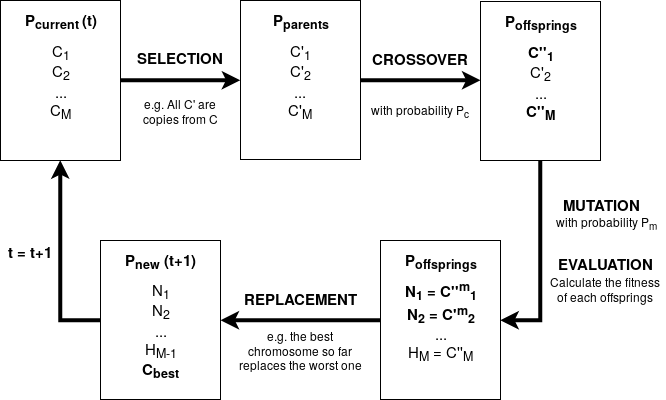
\includegraphics[width=\linewidth]{assets/images/EA_diagram.png}
    \caption{Overview of all genetic operators for a Evolutionary Algorithm. Modified illustration from Dr. F. Herrera  class notes}
    \label{fig:EA_diagram}
\end{figure}

To find good solutions with this algorithm we have to keep a good balance between exploitation and diversification. 

On the one hand, the selection, crossover and replacement operators focus on the exploitation of solutions with a promising fitness value in order to optimize solutions within a specific region of the search space. 

On the other hand, mutation and initialization diversify by generating rather different solutions from the existing ones; by doing so, the algorithm is able to explore new regions of the search space as well as avoiding getting stuck in local optima.

\section{Distributed Systems}
A distributed system is a collection of independent computers that appears to its users as a single coherent system. \cite{dissis_def}.

\begin{figure}[h!]
\centering
    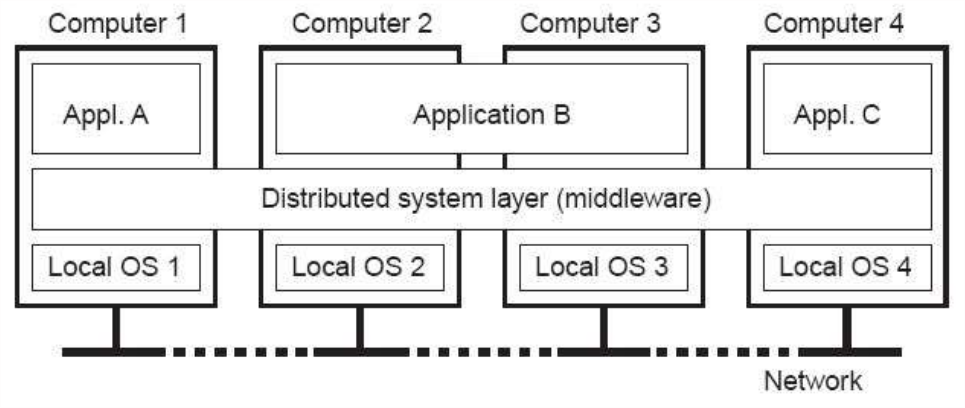
\includegraphics[scale=0.3]{assets/images/distributed-system_diagram.png}
    \caption{Distributed System from a user perspective}
    \label{fig:distributed_system}
\end{figure}

This collection of computers working as one needs to communicate, sharing information with each other in order to work towards the same objective. This exchange of communication can happen either by using shared memory or message passing.

Shared memory stands for memory that can be accessed concurrently by multiple programs. It is the fastest alternative but has two important disadvantages. The first one is that this alternative is expensive and does not scale well; it needs from these programs to be running within the same machine or at least be running in different machines that can share a common piece of hardware that stores the memory they share. The second main disadvantage of shared memory is that it is error prone; since multiple programs can access the same memory space, race conditions are likely to arise.

\begin{figure}[h!]
\centering
    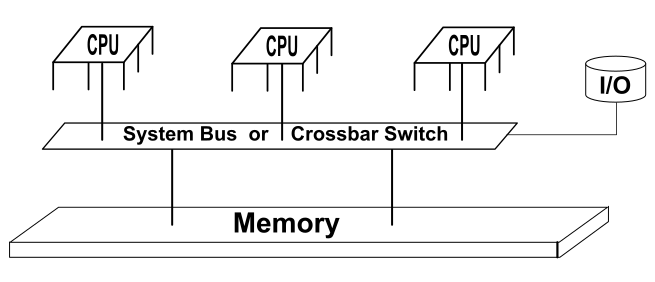
\includegraphics[scale=0.6]{assets/images/Shared_memory.png}
    \caption{Shared memory system of three processors}
    \label{fig:shared_memory}
\end{figure}

\newpage
Message passing is a method used to request behavior on a remote computer by sending an object containing enough information to select and run the appropriate code on the remote computer. this message passing can be synchronous if the requesting machine waits for the remote one to finish with the requested behavior, or asynchronous if it keeps busy on a different task. While synchronous systems are conceptually less complex, asynchronous ones usually achieve better performance.

Although this last approach comes with an overhead penalty due to data copying and delivery across machines, it is the best scaling one since interacting machines do not need to be close to each other to exchange information. Furthermore, because data sharing is explicit in message passing, there is less chance for errors to arise. 

\subsection{CAP Theorem}
The CAP Theorem states that it is impossible for any distributed system to simultaneously provide consistency, availability and partition tolerance. Only two out of these three properties can be provided at the same time\cite{wikipedia_cap}.

With the aim of easily explaining what these three properties are, as well as demonstrating this theorem, we will take an illustrated example\cite{cap-example} from the personal blog of \textit{Michael Whittaker}, a researcher from UC Berkeley.

\begin{wrapfigure}{r}{0.3\textwidth}
\centering
    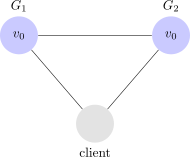
\includegraphics[width=0.25\textwidth]{assets/images/cap1.png}
    \caption{Example distributed system}
    \label{fig:dis-sys-1}
\end{wrapfigure}

Given a distributed system with two servers, $G_{1}$ and $G_{2}$, that can communicate with each other and are in charge of storing the value for a variable $v$ initialized to $v_{0}$. An a client that can request to write or read $v$ to any server that will answer back.

In a consistent system (Figure \ref{fig:consisten_system}), any read operation must return the latest written value within the whole system. In our example, if the client writes a new value $v_{1}$ for $v$ in $G_{1}$, when the client later reads $v$ from $G_{2}$, the server must return $v_{1}$.
\begin{figure}[h!]
\centering
    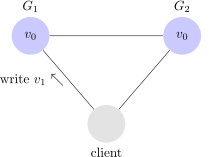
\includegraphics[scale=0.45]{assets/images/cap12.png}
    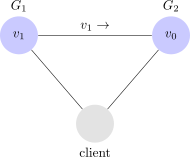
\includegraphics[scale=0.6]{assets/images/cap14.png}
    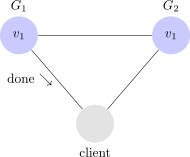
\includegraphics[scale=0.6]{assets/images/cap17.png}
    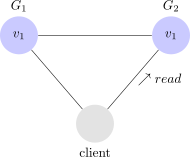
\includegraphics[scale=0.6]{assets/images/cap18.png}
    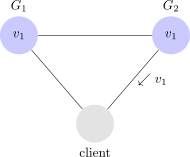
\includegraphics[scale=0.6]{assets/images/cap19.png}
    \caption{A consistent system}
    \label{fig:consisten_system}
\end{figure}

A distributed system offers availability if every time a client request is received by a non-failing server, it answers back.

Finally partition tolerance is achieved by the system when it is able to behave as expected if the network is allowed to lose arbitrarily many messages sent from one server to another.

To demonstrate this theorem, consider the system from Figure \ref{fig:non-cap-system} that provides consistency, availability and partition tolerance. When a client writes $v_{1}$ on $G_{1}$, because our system is always available it will respond. But, since it is partitioned, $G_{1}$ cannot replicate the new written value of $v$ to $G_{2}$. If the client now reads $v$ from $G_{2}$ will get $v_{0}$ as a response, making the system inconsistent.
\begin{figure}[h!]
\centering
    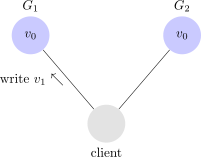
\includegraphics[scale=0.6]{assets/images/cap22.png}
    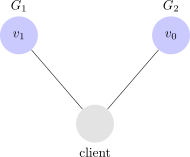
\includegraphics[scale=0.6]{assets/images/cap23.png}
    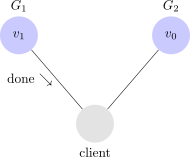
\includegraphics[scale=0.6]{assets/images/cap24.png}
    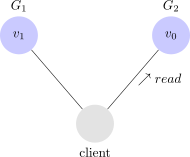
\includegraphics[scale=0.6]{assets/images/cap25.png}
    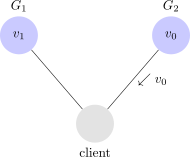
\includegraphics[scale=0.6]{assets/images/cap26.png}
    \caption{A partition tolerant and available system}
    \label{fig:non-cap-system}
\end{figure}

\subsection{Well known distributed architectures}
There are many different taxonomies for distributed systems architectures, but the following one is the most general and useful one to better understand this project in the following chapters.

\subsubsection*{Client-Server}
In this type of distributed system, we can distinguish two main components. The server, that process requests, and the clients, where the user requests services and resources from the servers. Examples of computer applications that uses this architecture are \textit{FTP}, \textit{Email}, or a \textit{Website}.

\begin{figure}[h!]
\centering
    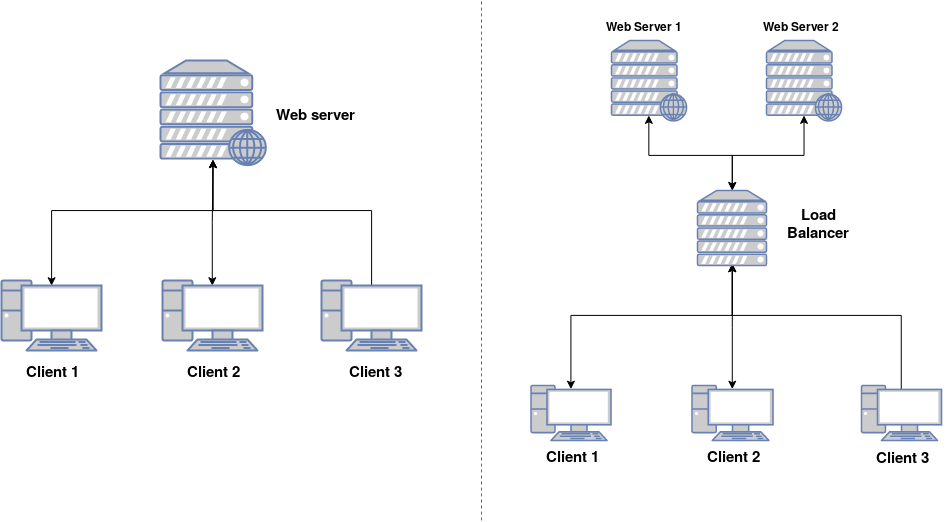
\includegraphics[width=\linewidth]{assets/images/client-server.png}
    \caption{Client-Server architecture. Left, simple approach. Right, with load-balancing}
    \label{fig:client-server}
\end{figure}

The main disadvantages of this architecture is that it has a single point of failure and scales poorly than other architectures since usually only one server handles all the requests from the clients. The scalability problem can be reduced by using load-balancing, where client requests are spitted among various servers that are able to handle these requests (Figure \ref{fig:client-server}).

\subsubsection*{Peer-to-peer}
Shortened as \textit{P2P}, it is a distributed system model where no central coordination by a server or stable hosts is needed. Instead, all responsibilities are uniformly divided among all machines, known as peers. Peers can serve both as clients and as servers\cite{p2p-principles}.
The first popular Peer-to-Peer system was Napster, a file-sharing service focused on music consumption.

Peer-to-peer networks implements a virtual network in the application layer that acts as an abstraction over lower layers of the actual networking model. This makes the P2P system independent from the physical network topology. Depending on how peers are connected to each other within the virtual network, we can classify these networks in two categories.

\begin{itemize}
    \item \textbf{Unstructured networks:} There is no particular structure on the virtual networks. When a new peer joins the system, it randomly connects to an already existing peer. This kind of networks scales well with a high rate of peers joining and leaving, but when a peer needs to find a particular resource in the network, there is an important increase of traffic within the network.\cite{structured-p2p}    
    
    \item \textbf{Structured networks:} The virtual network follows a specific topology where peers maintain a list of neighbors in order to route requests efficiently though the network. Although it enables the system to lookup for resources faster, it also makes the system less robust against a high rate of peers joining and leaving. It is the case of Distributed Hash Tables (DHT)\cite{dht}, which implements consistent hashing to assign ownership of resources to peers in the network and maintains a list of neighbors called \textit{finger-table} (Figure \ref{fig:dht}) that allows any node to find a resource in a logarithmic time.
    
\begin{figure}[h!]
\centering
    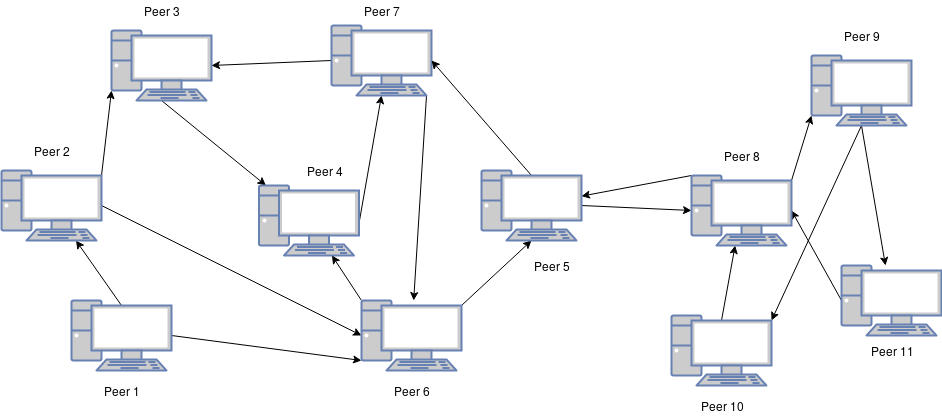
\includegraphics[width=\linewidth]{assets/images/p2p.png}
    \caption{Example of unstructured network}
    \label{fig:client-server}
\end{figure}    
    
\end{itemize} 
\begin{figure}[h!]
        \centering
        \begin{subfigure}{.5\textwidth}
          \centering
          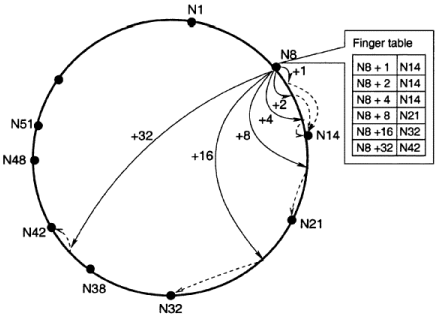
\includegraphics[width=\linewidth]{assets/images/dht1.png}
          \caption{}
          \label{fig:sub1}
        \end{subfigure}%
        \begin{subfigure}{.5\textwidth}
          \centering
          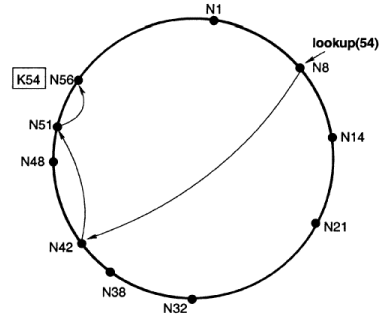
\includegraphics[width=\linewidth]{assets/images/dht2.png}
          \caption{}
          \label{fig:sub2}
        \end{subfigure}
        \caption{(a) Finger table of a DHT. (b) Lookup of resource with key $54$. \cite{dht_image}}
        \label{fig:dht}
    \end{figure}


\subsubsection*{Hybrid P2P Systems}
This architecture is a mixture of both Client-Server and Peer-to-Peer systems where certain functionalities are provided by servers. This approach enables the developer to make trade-offs between the advantages of using a centralized approach that is easier to maintain and develop, and using a peer-to-peer unstructured network.

This model often achieves better performance than pure Client-Server or Peer-to-Peer. Since certain functions that tends to create high networking traffic in a P2P system can by avoided using a centralized approach.

A good example of system using this approach is BitTorrent\cite{bittorrent} (Figure \ref{fig:bittorrent}). With a Client-Server model, \textit{tracker} servers and \textit{torrent} repositories provides a structured virtual network, while the rest of nodes constitute the unstructured network with a Peer-to-Peer approach.

\begin{figure}[h!]
    \centering
    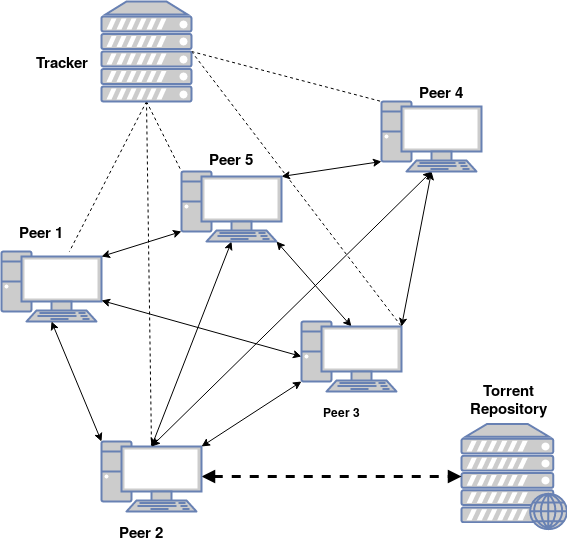
\includegraphics[width=0.5\linewidth]{assets/images/bittorrent.png}
    \caption{BitTorrent Network}
    \label{fig:bittorrent}
\end{figure}  


\section{Technosocial Systems}
\begin{quote}
\textit{Technosocial Systems are people and technologies that combine to work as heterogeneous but functional wholes.}
    \begin{flushright}
        \tiny{--- Edward Woodhouse and Jason W. Patton \cite{technosocial}}
    \end{flushright}
\end{quote}

At the beginning of the 21st century, the web started shifting from static data that is read-only for consumers to a more complex and dynamic paradigm where communication between users is the main objective. The best example to showcase this transformation is social networks, where users generate the content that is subsequently consumed by other users.

At the same time, although with a slower pace, an even more advanced web paradigm is emerging. Build on top of the communication-oriented model previously described, this paradigm is characterized by co-operation between users of a platform towards a common goal. 

Examples of successful communities that follow this paradigm are \textit{Wikipedia}, where users actively contribute with the objective of creating a free-access encyclopedia. And \textit{Schema.org}, with the mission to create structured data on the Internet that is computer-understandable.

This project falls into the last category by enabling cooperation between users of the platform towards the common goal of solving difficult problems that need from a high computing power to be addressed.




































